\begin{frame}
\frametitle{Deadlock}
\begin{itemize}
    \item<1->Deadlock - ситуация, при которой потоки не могут работать,
         потому что ждут друг друга:
    \begin{itemize}
        \item<2->deadlock потоком исполнения и обработчиком прерывания;
        \item<3->поток A ждет, пока поток B что-то сделает (например, отпустит
             блокировку);
        \item<4->а поток B ничего не делает, потому что ждет, пока поток A
             что-то сделает (например, отпустит блокировку).
    \end{itemize}
\end{itemize}
\end{frame}

\begin{frame}[fragile]
\frametitle{Пример}
\begin{columns}
    \begin{column}{.35\textwidth}
        \begin{lstlisting}
struct lock a;

void thread0(void)
{
    lock(&a);
    lock(&b);

    /* do something */

    unlock(&a);
    unlock(&b);
}
        \end{lstlisting}
    \end{column}
    \begin{column}{.35\textwidth}
        \begin{lstlisting}
struct lock b;

void thread1(void)
{
    lock(&b);
    lock(&a);

    /* do something else */

    unlock(&a);
    unlock(&b);
}
        \end{lstlisting}
    \end{column}
    \begin{column}{.3\textwidth}
    \end{column}
\end{columns}
\end{frame}

\begin{frame}[fragile]
\frametitle{Пример}
\begin{columns}
    \begin{column}{.35\textwidth}
        \begin{lstlisting}
    lock(&a);

    lock(&b);

        \end{lstlisting}
    \end{column}
    \begin{column}{.35\textwidth}
        \begin{lstlisting}

    lock(&b);

    lock(&a);
        \end{lstlisting}
    \end{column}
    \begin{column}{.3\textwidth}
    \end{column}
\end{columns}
\end{frame}

\begin{frame}
\frametitle{Wait-for граф}
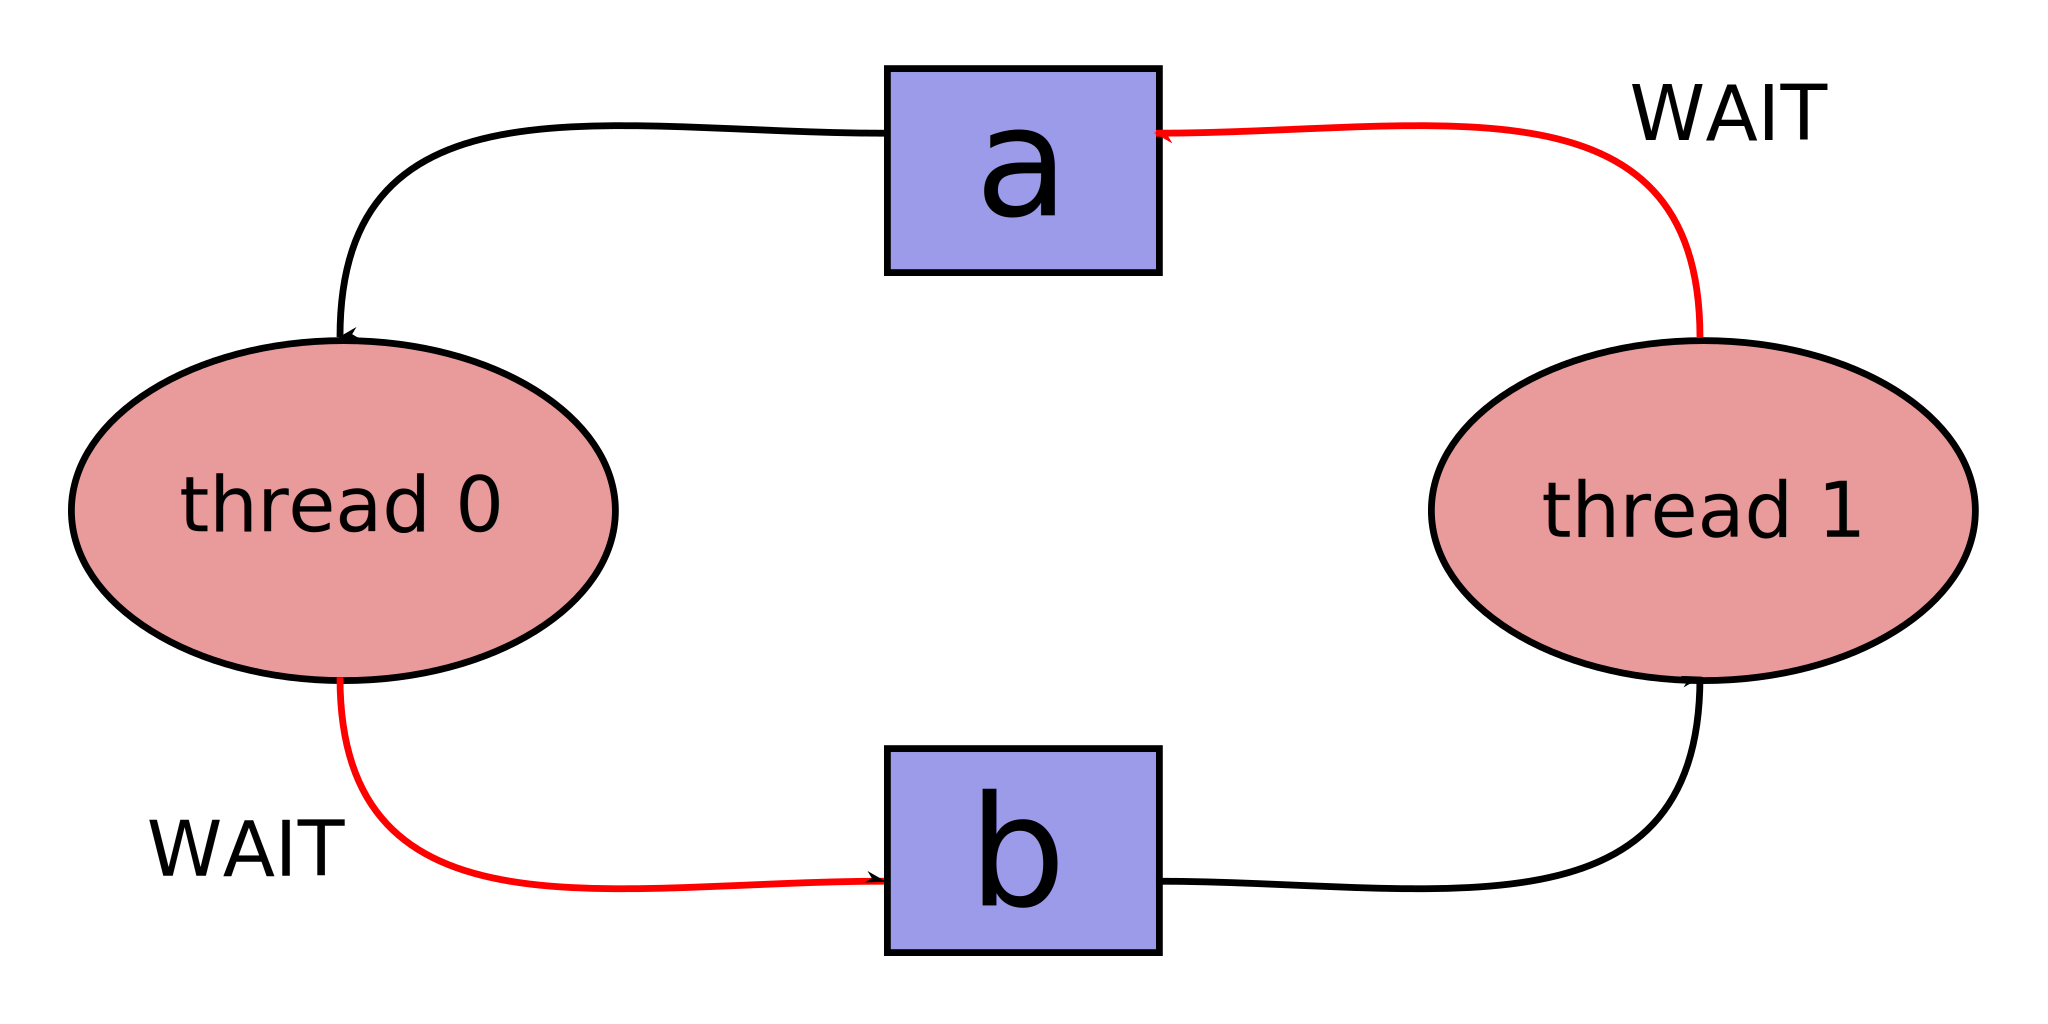
\includegraphics[height=.4\textheight]{waitfor}
\end{frame}

\begin{frame}
\frametitle{Deadlock}
\begin{itemize}
    \item<1->Как и с состоянием гонки, deadlock не поддается тестированию
    \begin{itemize}
        \item<2->появление зависит от многих факторов;
        \item<3->входные данные, решения планировщика, прерывания,
             производительность оборудования ...
    \end{itemize}
\end{itemize}
\end{frame}

\begin{frame}
\frametitle{Предотвращение deadlock-ов}
\begin{itemize}
    \item<1->Мы хотим избежать появления цикла в wait-for графе
    \begin{itemize}
        \item<2->простой случай - все блокировки известны заранее;
        \item<3->упорядочим все блокировки (например, по адресу);
        \item<4->захватываем блокировки только по порядку.
    \end{itemize}
\end{itemize}
\end{frame}

\begin{frame}[fragile]
\frametitle{Пример}
\begin{columns}
    \begin{column}{.35\linewidth}
        \begin{lstlisting}
void thread0()
{
    lock(&a);
    lock(&b);
    ...
    unlock(&b);
    unlock(&a);
}
        \end{lstlisting}
        \begin{lstlisting}
void thread2()
{
    lock(&c);
    lock(&a);
    ...
    unlock(&a);
    unlock(&c);
}
        \end{lstlisting}
    \end{column}
    \begin{column}{.35\linewidth}
        \begin{lstlisting}
void thread1()
{
    lock(&b);
    lock(&c);
    ...
    unlock(&c);
    unlock(&b);
}
        \end{lstlisting}
    \end{column}
    \begin{column}{.3\linewidth}
    \end{column}
\end{columns}
\end{frame}

\begin{frame}
\frametitle{Пример}
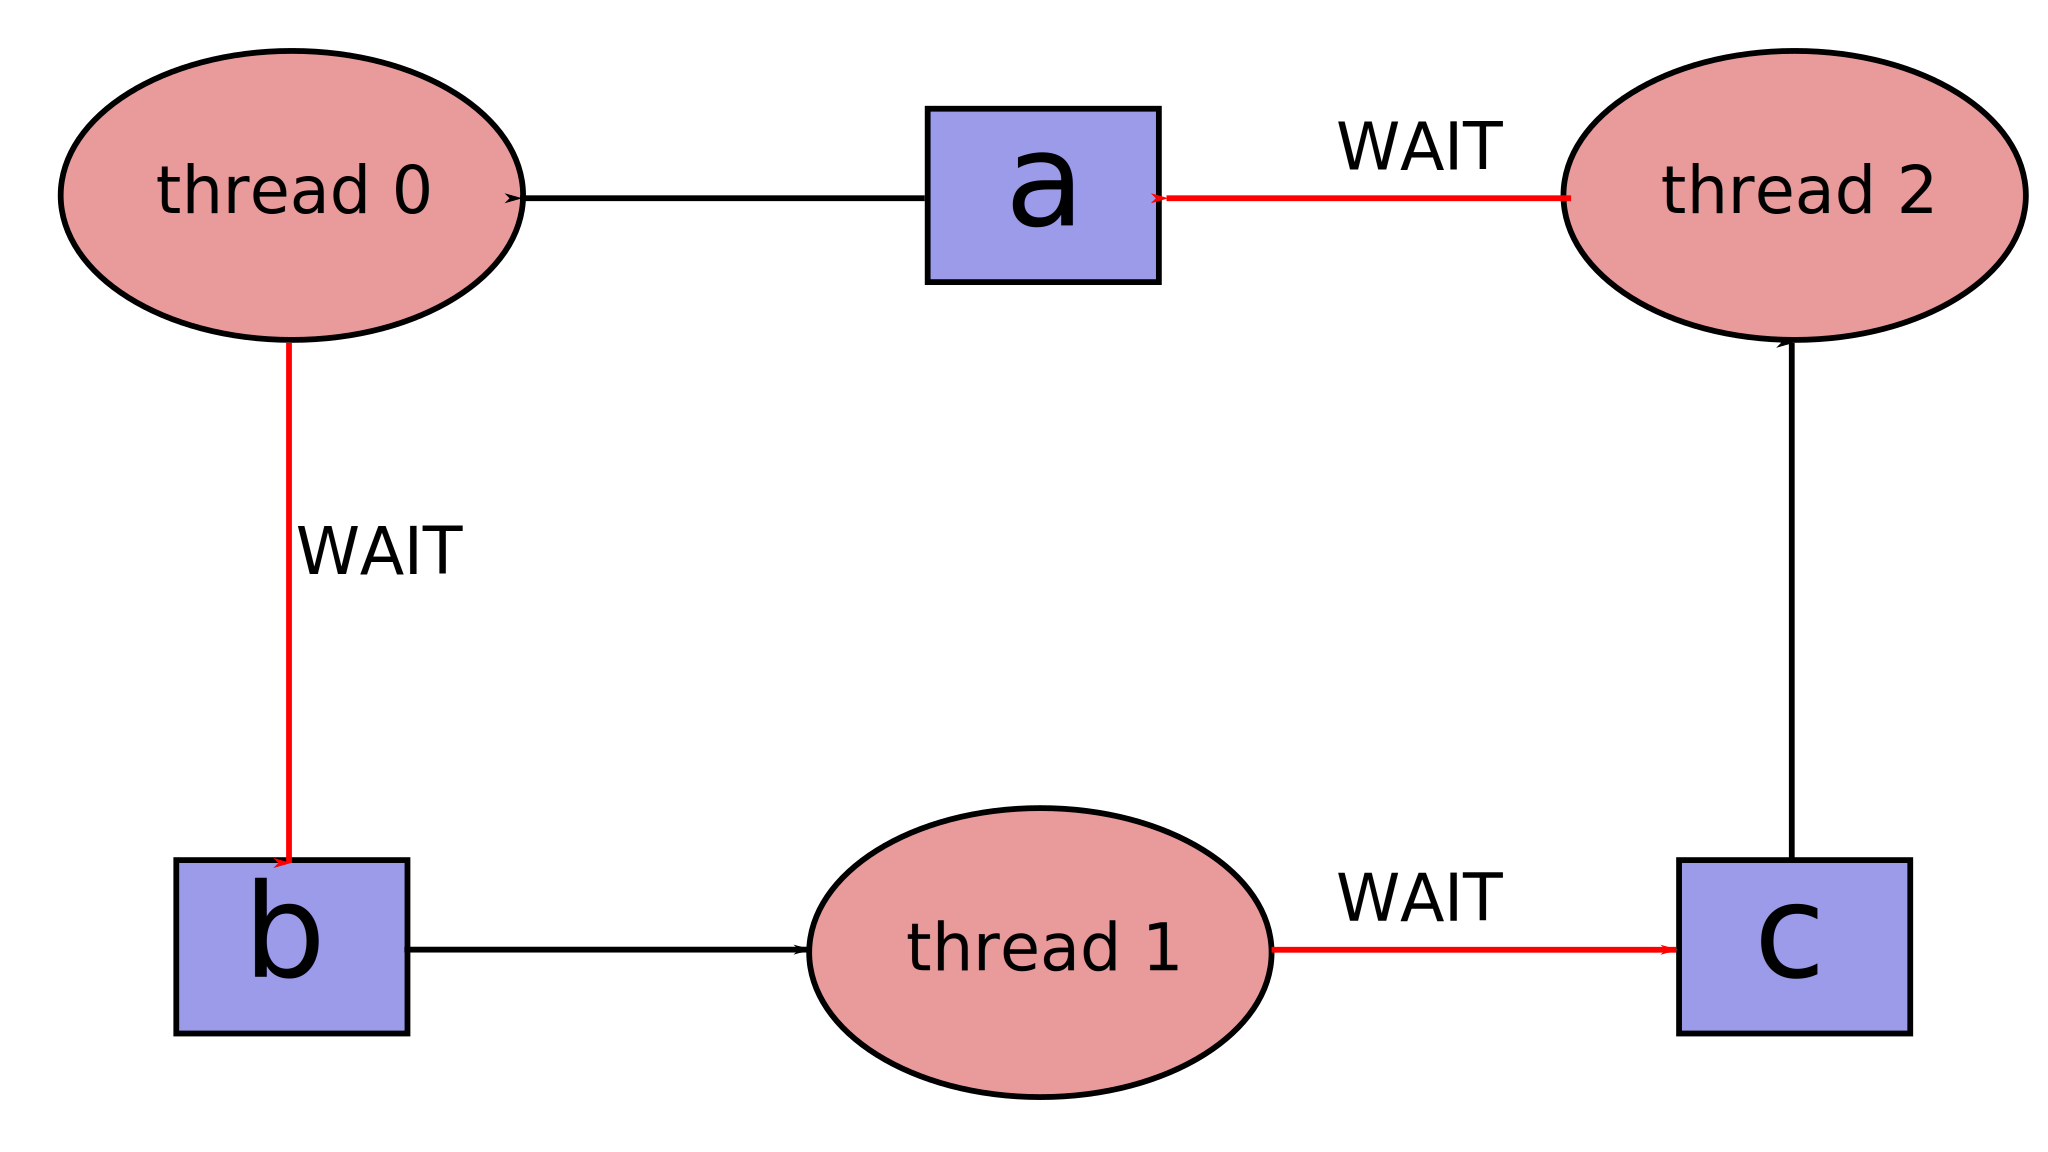
\includegraphics[height=.4\textheight]{order}
\end{frame}

\begin{frame}
\frametitle{Пример}
\begin{itemize}
    \item<1->Отсортируем блокировки a, b и c по алфавиту:
    \begin{itemize}
        \item<2->каждый поток должен захватывать блокировки только согласно
             порядку;
        \item<3->например, поток 2 хочет захватить блокировки c и a:
        \begin{itemize}
            \item<4->так как a в алфавтие раньше c, то сначала хватаем a,
            \item<5->потом хватаем c.
        \end{itemize}
    \end{itemize}
\end{itemize}
\end{frame}

\begin{frame}[fragile]
\frametitle{Пример}
\begin{columns}
    \begin{column}{.35\linewidth}
        \begin{lstlisting}
void thread0()
{
    lock(&a);
    lock(&b);
    ...
    unlock(&b);
    unlock(&a);
}
        \end{lstlisting}
        \begin{lstlisting}
void thread2()
{
    lock(&a);
    lock(&c);
    ...
    unlock(&c);
    unlock(&a);
}
        \end{lstlisting}
    \end{column}
    \begin{column}{.35\linewidth}
        \begin{lstlisting}
void thread1()
{
    lock(&b);
    lock(&c);
    ...
    unlock(&c);
    unlock(&b);
}
        \end{lstlisting}
    \end{column}
    \begin{column}{.3\linewidth}
    \end{column}
\end{columns}
\end{frame}

\begin{frame}
\frametitle{Предотвращение deadlock-ов}
\begin{itemize}
    \item<1->Сложный случай - все блокировки не известны заранее:
    \begin{itemize}
        \item<2->для этого случая придумано много различных вариантов;
        \item<3->мы рассмотрим подход, который называется Wait-Die.
    \end{itemize}
\end{itemize}
\end{frame}

\begin{frame}[fragile]
\frametitle{Изменим интерфейс}
\begin{lstlisting}
    struct wdlock_ctx {
        unsigned long long timestamp;
	struct wdlock *next;
    };

    struct wdlock {
        ...
    };

    /* Grab unique "timestamp" */
    void wdlock_ctx_init(struct wdlock_ctx *ctx);

    /* This function may fail */
    int wdlock_lock(struct wdlock *lock,
                    struct wdlock_ctx *ctx);

    /* Unlocks all of the locks */
    void wdlock_unlock(struct wdlock_ctx *ctx);
\end{lstlisting}
\end{frame}

\begin{frame}[fragile]
\frametitle{Как использовать Wait-Die подход?}
\begin{lstlisting}
    void thread(void)
    {
        struct wdlock_ctx ctx;

        wdlock_ctx_init(&ctx);

        while (1) {
            ...
            if (!wdlock_lock(&lock1, &ctx)) {
                wdlock_unlock(&ctx);
                continue;
            }
            ...
            if (!wdlock_lock(&lock2, &ctx)) {
                wdlock_unlock(&ctx);
                continue;
            }
            ...
        }
        /* Acquired all required locks successfully,
           can do something. */
        wdlock_unlock(&ctx);
    }
\end{lstlisting}
\end{frame}

\begin{frame}
\frametitle{"Контекст"}
\begin{itemize}
    \item<1->Wait-Die контекст состоит из:
    \begin{itemize}
        \item<2->списка захваченных блокировок;
        \item<3->уникального "timestamp".
    \end{itemize}
\end{itemize}
\end{frame}

\begin{frame}[fragile]
\frametitle{"Контекст"}
\begin{lstlisting}
    struct wdlock_ctx {
        unsigned long long timestamp;
	struct wdlock *next;
    };


    void wdlock_ctx_init(struct wdlock_ctx *ctx)
    {
        static atomic_ullong timestamp;

        ctx->timestamp = atomic_fetch_add(&timestamp, 1) + 1;
        ctx->next = NULL;
    }
\end{lstlisting}
\end{frame}

\begin{frame}
\frametitle{Магия timestamp}
\begin{itemize}
    \item<1->timestamp позволяет избегать deadlock-ов
    \begin{itemize}
        \item<2->храним в каждой блокировке timestamp из wdlock\_ctx, который
             использовали при захвате блокировки;
        \item<3->при попытке захватить блокировку возможно несколько вариантов:
        \begin{itemize}
            \item<4->если блокировка свободна, то пытаемся ее захватить - как
                 обычно;
            \item<5->если блокировка занята, то нужно сравнить timestamp-ы.
        \end{itemize}
    \end{itemize}
\end{itemize}
\end{frame}

\begin{frame}
\frametitle{Магия timestamp}
\begin{itemize}
    \item<1->Если блокировка захвачена, то нужно сравнить наш timestamp с
         сохраненным в блокировке:
    \begin{itemize}
        \item<2->если наш timestamp меньше, чем timestamp блокировки, то ждем;
        \item<3->в противном случае не ждем, а возвращаем признак неудачи
             (умираем).
    \end{itemize}
\end{itemize}
\end{frame}

\begin{frame}
\frametitle{Корректность}
\begin{itemize}
    \item<1->Поток ждет на блокировке, если timestamp блокировки больше,
         чем timestamp потока
    \begin{itemize}
        \item<2->deadlock соответствует циклу в Wait-For графе;
        \item<3->при использовании Wait-Die timestamp-ы блокировок на любом
             пути в графе строго возрастают;
        \item<4->следовательно, цикла в Wait-For графе быть не может.
    \end{itemize}
\end{itemize}
\end{frame}

\begin{frame}
\frametitle{Wait-Die граф}
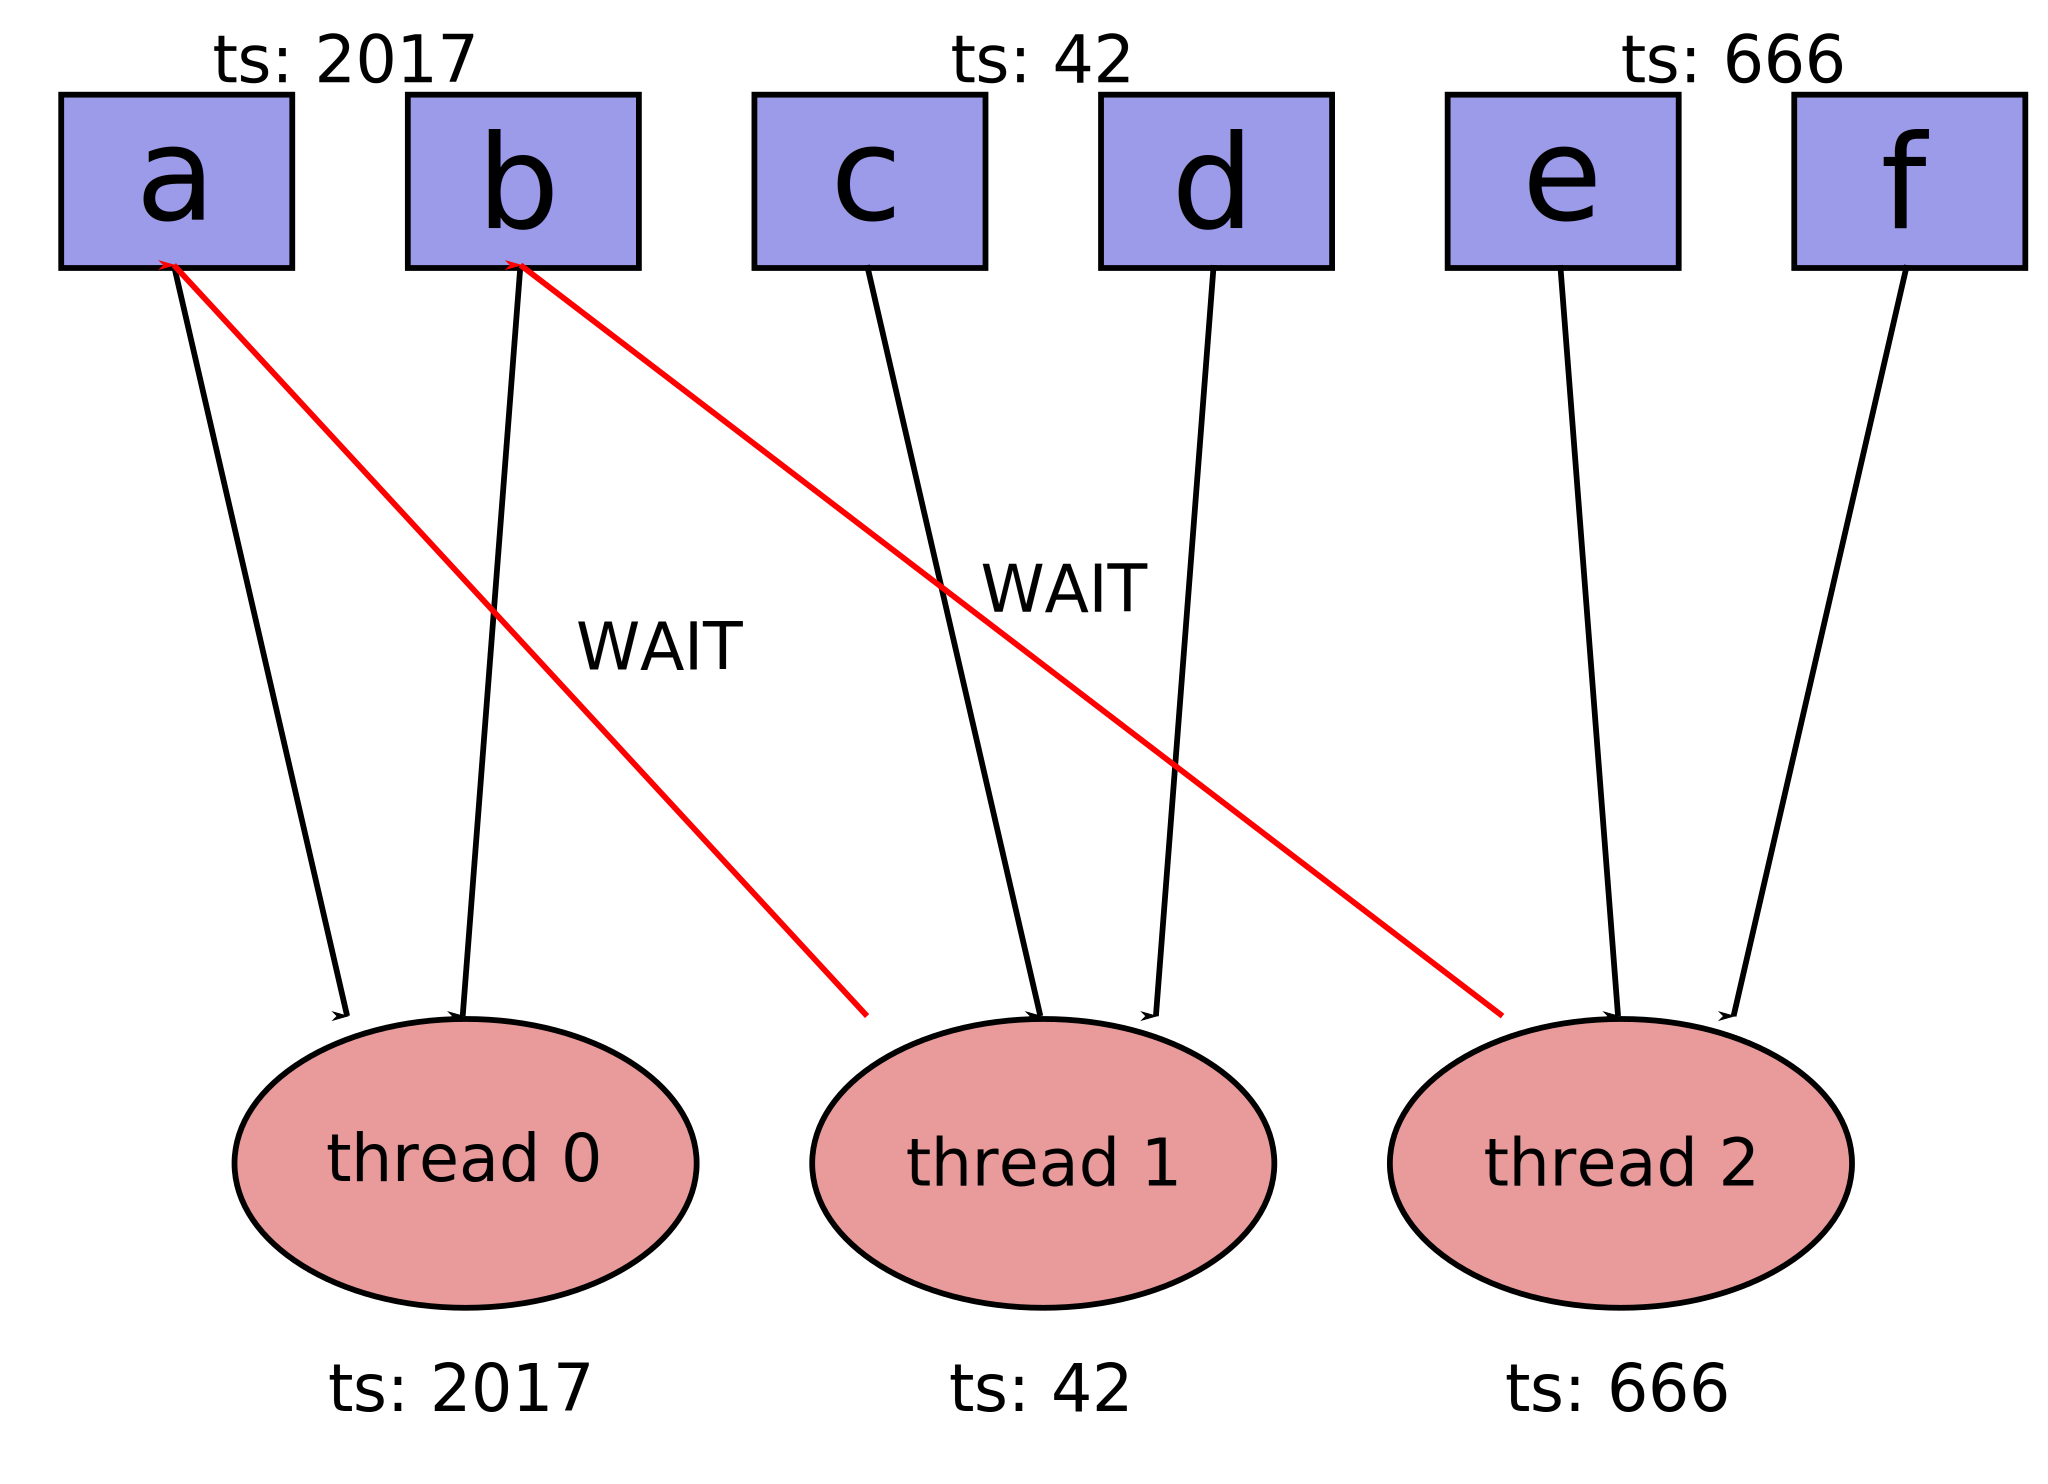
\includegraphics[height=.4\textheight]{waitdie}
\end{frame}

